\section{Collaborative ML Workload Optimizations} \label{sec-ml-workloads}
\hladd{
In this section, we first define the required terms which refer to different entities in collaborative data science platforms. 
Then, we discuss the details of the experiment graph construction and workflow of our system and optimization process.
Finally, we show how a real collaborative data science platform can utilize our system to improve the execution of machine learning workloads.
}

\subsection{Preliminaries and Definitions}
\hladd{
\textbf{ML Task.} 
In order to promote a collaborative effort, collaborative data science platforms must define the task which the users should solve.
A task specifies the requirements and the goal of machine learning solutions.
In our system, the definition of an ML task contains the following.
(1) The type of the machine learning model, i.e., classification, regression, or clustering.
(2) One or multiple datasets grouped into training and test (except for unsupervised tasks, which do not require a test dataset).
(3) An evaluation function which assigns a score to the user-provided solution.
An example of a task is to train a classification model on the training dataset $D_1$ which maximizes the F1 score on the evaluation test dataset $D_2$.
%For example, in Kaggle, a task corresponds to a competition with a predefined set of training datasets, testing datasets, and an evaluation function.

\textbf{ML Workload Data and Operations.}
In our system, we support three types of data.
(1) A \textit{Dataset} which has one or more columns of data and is analogous to dataframe objects (e.g., pandas dataframe \cite{mckinney-proc-scipy-2010}).
(2) An \textit{Aggregate} which contains a single value or list of values.
(3) A \textit{Model} which represents a trained machine learning model.

Each data type results from one of the following three types of operations.
(1) Data preprocessing and feature engineering operations which include simple data transformation and aggregation, feature selection, and feature extraction operations.
This group of operations either return another Dataset (e.g., resulting from map, filter, or one-hot encoding) or an Aggregate (e.g., resulting from reduce or column correlation).
(2) Model training operations which train a machine learning model on a Dataset.
The result of model training operations can either be used in other data and feature engineering operations (e.g., a PCA model) or can be used to perform prediction on a test dataset.
Model training operations return a Model type.
(3) Hyperparameter tuning operations which have the task of finding the best hyperparameters for a machine learning model.
The most common tuning approaches are grid search, random search, and Bayesian hyperparameter search \cite{bergstra2012random,snoek2012practical}.
In all three approaches, several models with different hyperparameters are trained and the model which performs the best is returned as the final result.
In our system, instead of only returning the best performing model, we also capture all the runs with different hyperparameters.
As a result, hyperparameter tuning operations returns a set of Models.
 
\textbf{ML Workload Type.}
Collaborative data science platforms typically provide two modes of executions for solving tasks:
\textit{long-running workloads} and \textit{interactive workloads}.
The user can write an end-to-end script which performs data loading, data cleaning, and model training. We refer to this type of workloads as long-running workloads.
Depending on the size of the initial data, a long-running workload may take anything from seconds up to many hours.
The other type of workloads is more interactive.
Typically, through Jupyter notebooks, collaborative data science platforms allow users to write their analysis in an interactive fashion, whereupon execution of each operation (or group of operations), they can view the result and fine-tune their analysis code.
We refer to this type of workloads as interactive workloads.
}

\subsection{Experiment Graph Representation}\label{sub-graph-construction}
\textbf{Workload DAG.}
A machine learning workload can be represented using a directed acyclic graph (DAG).
In the DAG, vertices represent the artifacts, i.e., raw or preprocessed data (represented by data frame objects) and machine learning models resulting from feature engineering and model training operations and edges represent the operations in the workload.
Each workload DAG has one or more initial vertices representing the raw datasets which are defined as part of the task definition in a collaborative platform.
We refer to the initial vertices as the roots.

\textbf{Experiment Graph. }
For every task, the collection of all the DAGs of the previously executed machine learning workloads forms a rooted graph (with potentially multiple root vertices) which we refer to as the \textit{experiment graph}.
More formally, we represent the experiment graph by $G(V, E)$.
$V=\{v_i\}, i = 1, \cdots, n$ is the set of all the artifacts in all the workload DAGs.
$E=\{e_i\}, i = 1, \cdots, m$ is the set of all the executed operations in the workload DAGs.
A directed edge $e$ from $v_i$ to $v_j$ in $G(V, E)$ indicates that the artifact $v_j$ is derived from the artifact $v_i$ by applying the operation in $e$.
Every vertex $v$ has the attributes $\langle f, s \rangle$ (accessed by $v.f$ and $v.s$) which represent the frequency, i.e., number of different workloads an artifact appeared in, and storage size of the artifact.
Every edge $e$ has the attribute $\langle t \rangle$ (accessed by $e.t$) which represents the run-time (in seconds) of the operation.

Inside each vertex, we store the meta-data of the artifact.
Depending on how \textit{useful} an artifact is, we may also store the actual underlying data inside the artifact (Section \ref{sec-materialization}).
If the artifact is a raw or a preprocessed dataset, then its meta-data includes the name, type, and total size of each column of the data and its underlying data is represented by the dataframe object (i.e., pandas dataframe \cite{mckinney-proc-scipy-2010}). 
If the artifact is a machine learning model, its meta-data includes the name, type, hyperparameters, and the error metric of the model and its underlying data is consist of the model weights.
Each edge contains the meta-data of the operation it represents, such as the function name, training algorithm, hyperparameters, and in some cases even the source code of the operation.
To uniquely identify an edge, we utilize a hash function which receives as input the operation and its hyperparameters (if it has any).
Since the experiment graph is rooted, we assign a hash value to every vertex which is computed in the following way:
\[
    h(v)= 
\begin{cases}
    id,& \text{if } v \text{ is root}\\
    h\Big(\sum\limits_{e \in in\_edge(v)} (h(e.source) + h(e) ) \Big)  ,              & \text{otherwise}.
\end{cases}
\]
where $in\_edge(v)$ returns the edges with destination $v$. 
Intuitively, the hash of a root vertex is its unique identifier (location on disk or download URL) and the hashes of other vertices are derived by combining the hashes of their parents and edges which connect them to their parents.
%This hashing procedure results in two important properties.
%
%\textit{Property 1}.
%The two vertices, $v_1$ and $v_2$ in graphs $G_1$ and $G_2$ are the same if and only if $h(v_1)$ in $G_1$ is the same as $h(v_2)$ in $G_2$.
%
%\textit{Property 2}.
%If a vertex $v_1$ in graph $G_1$ does not exist in $G_2$ , then no successors of $v_1$ can exist in $G_2$.}

After a machine learning workload is executed, we update the experiment graph by adding the new artifacts and operations.
If any of the artifacts already exist in the graph, their frequency is updated.

\hladd{
\textbf{Workload DAG generation.}
Instead of designing a new DSL, we extend the existing pandas \cite{mckinney-proc-scipy-2010} and scikit-learn \cite{sklearn_api} python packages which are frequently used for data analysis and machine learning workloads.
Listing \ref{listing-experiment-graph} shows an example of a workload script.
With only a slight modification of the import commands, we are able to load our system's modules.
A parser component reads the user code and instead of executing it line-by-line, it creates the edges and vertices of the workload DAG.
The actual execution is invoked with \textit{.get()} command of a vertex (Line 18, Listing \ref{listing-experiment-graph}.
}
Figure \ref{fig-experiment-graph}a shows an example graph constructed from the code in Listing  Listing \ref{listing-experiment-graph}.
\begin{figure}
\begin{subfigure}[b]{0.4\linewidth}
\centering
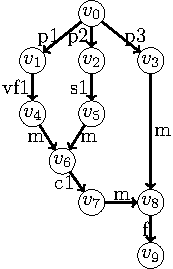
\includegraphics[width=0.8\linewidth]{../images/tikz-standalone/example-graph}
\caption{}
\end{subfigure}%
\begin{subfigure}[b]{0.6\linewidth}
\begin{tabular}{lcl}
\hline
operation & label &  hash \\
\hline
project(ad..) & $\langle 2s\rangle$ &p1 \\
project(ts, ..) & $\langle 6s\rangle$ & p2\\
project(y) & $\langle 2s\rangle$ & p3\\
vectorizer.f\_t & $\langle 40s\rangle$ & vf1 \\
selector.f\_t & $\langle 60s\rangle$ & s1 \\
concat & $\langle 10s\rangle$ & c1 \\
merge & $\langle 0s\rangle$ & m\\
svm.fit & $\langle 100s\rangle$ & f\\
\hline
\end{tabular}
\caption{}
\end{subfigure}
\caption{Experiment graph constructed from the Listing \ref{listing-experiment-graph} (a) and the hash of the operations in the scripts (b)}
\label{fig-experiment-graph}
\end{figure}
Table \ref{fig-experiment-graph}b shows both the label of every edge operation, i.e., time, and the hash of the operations and their hyperparameters.

\begin{lstlisting}[language=Python, caption=Example script,captionpos=b,label = {listing-experiment-graph}]
import custom_pandas as pd

from custom_sklearn import svm
from custom_sklearn.feature_selection import SelectKBest
from custom_sklearn.feature_extraction.text import CountVectorizer

train = pd.read_csv('../input/train.csv') 
print train.columns # [ad_desc,ts,u_id,price,y]
vectorizer = CountVectorizer()
count_vectorized = vectorizer.fit_transform(train['ad_desc'])
selector =  SelectKBest(k=2)
top_features = selector.fit_transform(
                                  train[['ts','u_id','price']],  
                                  train['y'])
top_features # print the content of the data frame			     
X = pd.concat([count_vectorized,top_features], axis = 1)
model = svm.SVC().fit(X, train['y'])
model.get()
\end{lstlisting}

Since at the time of the execution of the script, the experiment graph is empty, all the artifacts (vertices) have a frequency of 1.
In order to represent operations which process multiple input artifacts, e.g., concat and svm.fit operations in Listing \ref{listing-experiment-graph}, we proceed as follows.
First, we merge the vertices representing the artifacts into a single vertex using a merge operator.
The merge operator is a logical operator which does not incur a cost, i.e., it has a run-time of 0 seconds.
The merged vertex is also a logical vertex with no actual attributes which only contains the vertex ids of the merged vertices.
Then, we draw an edge from the merged vertex which represents the actual operation.
For example, in Figure \ref{fig-experiment-graph}a, before applying the concatenation operation, we merge $v_4$ and $v_5$ into $v_6$, then we apply the concatenation operation (c1).
Furthermore, when computing the hash of a merged vertex, we take the merge order into account.
For example, the operation svm.fit has $X$ (represented by $v_7$) as first argument and train['y'] (represented by $v_3$) as its second argument.
When computing hash of $v_8$, we combine the parents in the same order, i.e., $h(v_8) = h(h(v_7) + m + h(v_3) + m)$. 
After the DAG is constructed, its execution is invoked with the call to the $get()$ command on Line 18.
\hladd{
\subsection{System Architecture and Workflow}
Figure \ref{system-workflow} shows the components of the collaborative workload optimizer system.
First, a parser component generates the workload DAG from the user scripts (Step 1).
Upon the invocation of the $get()$ method of an artifact, a local optimization process beings.
The local optimizer extracts the subgraph which must be executed in order to compute the terminal vertex.
The Local optimizer traverses the graph in reverse order starting at the terminal vertex until the root vertices.
It stops the traversal when it reaches a previously computed vertex.
In interactive workloads, it is likely that many of the intermediate vertices between the terminal vertex and the root vertices are previously computed.
The subgraph of all the visited vertices and the edges connecting them, which we refer to as the  \textit{local execution DAG}, is the result of the local optimizer (Step 2).
%For example in Figure \ref{system-workflow}, the traversal begins at Vertex 7 and continues until it visits Vertices 2 and 3.
%Since both Vertices are already computed (depicted with black color), the traversal stops and returns the subgraph starting at Vertices 2 and 3. 
The global optimizer component receives the local execution subgraph and looks for optimization opportunities, i.e., reusing materialized vertices or warmstarting model training, in the experiment graph.
The result of the global optimization process is another execution subgraph, which we refer to as the \textit{global execution subgraph} (Step 3).
%For example, in Figure \ref{system-workflow}, the experiment graph has previously materialized the underlying data (Dataset, Aggregate, or Model) of Vertex 5.
%Therefore, during the global optimization, the underlying data of Vertex 5 is transferred to the workload which results in another subgraph with Vertex 3 and Edge $e_4$ pruned.
Then, an execution planner receives the global execution subgraph and sorts the edges based on their topological order, which are then executed by the execution engine (Step 4).
After the execution, an updater component updates the experiment graph to include the vertices and edges of the workload DAG.
Furthermore, the updater component also decides what vertices to materialize, i.e., store their underlying data in the vertex of the graph (Step 5).

\begin{figure}
\centering
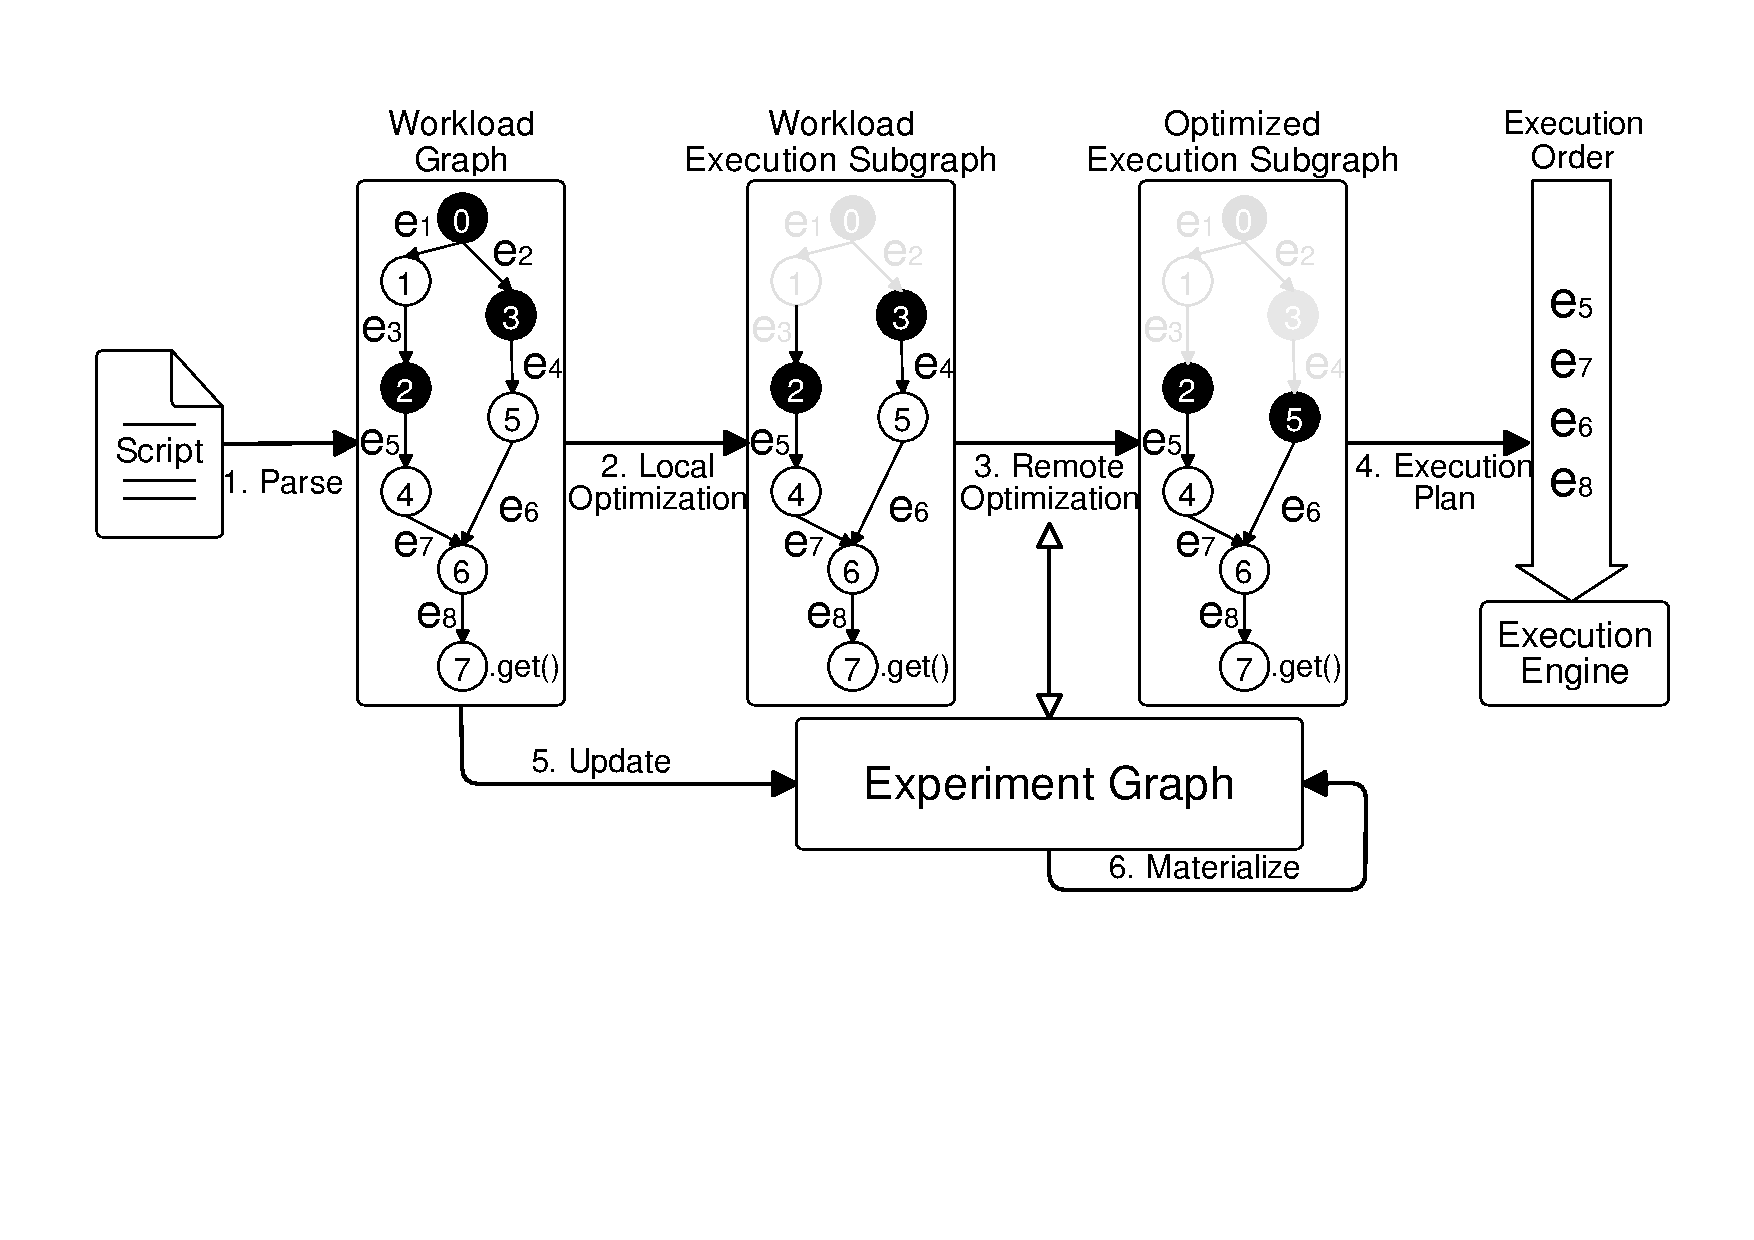
\includegraphics[width=\columnwidth]{../images/system-workflow}
\caption{System overview of the collaborative workload optimizer}
\label{system-workflow}
\end{figure}


\subsection{Workload Optimizer for Kaggle Use Case}
In this section, we describe how our system can be integrated into Kaggle's collaborative data science platform to improve the execution of the kernels.
We select the competition \textit{Home Credit Default Risk}\footnote{https://www.kaggle.com/c/home-credit-default-risk/}.
The task of the competition is to train a classification model which predicts whether a client is able to repay their loans.
The task has 8 training datasets and 1 test datasets.
The goal of the submitted solutions is to maximize the evaluation function, the area under the ROC curve between the predicted values and observed target values.
After a kernel is submitted, it goes through every step of the workload optimizer system in Figure \ref{system-workflow}.
For every competition, we maintain a separate experiment graph.
At the time of the first kernel submission, the experiment graph is empty, therefore, the workload optimizer system skips Step 3 of Figure \ref{system-workflow} and generates the execution plan directly from the workload execution subgraph.
If the experiment graph is not empty, the global optimizer tries to optimize the workload using the experiment graph.
For example, the most popular kernel\footnote{https://www.kaggle.com/willkoehrsen/start-here-a-gentle-introduction} in the competition has been copied by more than 5000 different users.
This indicates the kernel has been executed at least 5000 times, although it is very likely that many of the users run the script more than once.
Each execution of the kernel takes nearly 200 seconds.
In our experiments, we show that we are able to reduce the execution time to less than 10 seconds when the same kernel is executed more than once.
}
%
%First, we parse a kernel and construct the \textit{workload graph} (\circledtext{1}).
%Then, an \textbf{optimizer} component receives the workload graph and utilizes the existing experiment graph to look for optimization opportunities, namely, reusing the existing operations and warmstarting the model training (\circledtext{2}).
%The result of the optimization is another workload graph which contains precomputed artifacts and warmstarted models.
%After executing the optimized workload, we return the result to the user (\circledtext{3}).
%Depending on the number of \textit{pipeline subgraphs} in the workload, the result of the execution is one or multiple \textit{terminal models} which the user can choose to submit as their solution to the competition.
%After the execution, we update the experiment graph using the original workload graph (\circledtext{4}).
%Finally, to ensure that we can store the experiment graph given our storage budget, we execute our materialization algorithms to decide what artifacts to materialize (\circledtext{5}).
%
%\begin{figure}
%\centering
%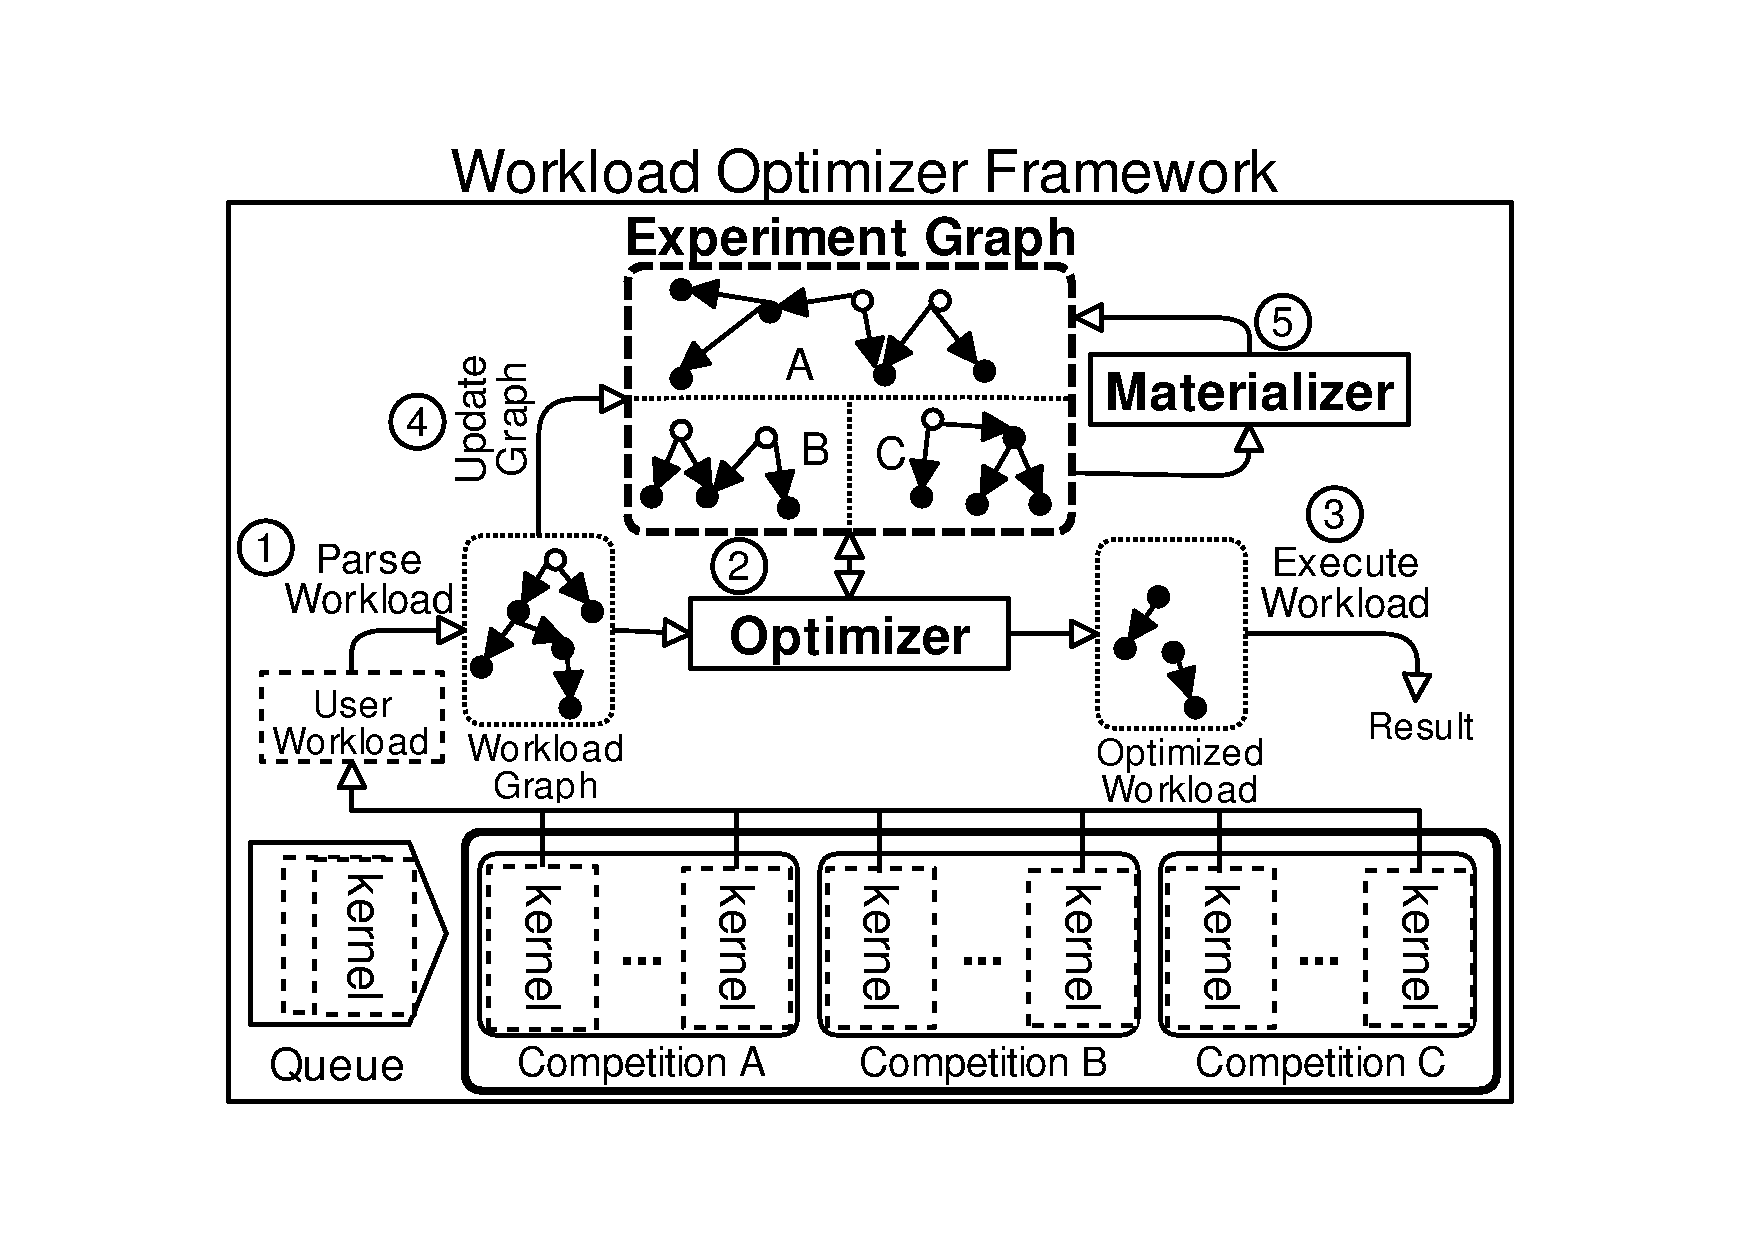
\includegraphics[width=\columnwidth]{../images/kaggle-workload-optimizer}
%\caption{Improving the execution of Kaggle Kernels with Workload Optimizer}
%\label{improved-use-case}
%\end{figure}
%
%In the experiment graph, each task corresponds to one connected component rooted at vertices representing the tasks root datasets.
%Since each task has unique roots and workloads are not allowed to analyze roots belonging to multiple tasks, it is impossible for two tasks to be connected.
%In Figure \ref{improved-use-case}, the experiment graph has three connected components representing the three competitions, A, B, and C which have 2, 2, and 1 root datasets, depicted as hollow vertices, respectively.
%When optimizing a new Kaggle kernel from competition A, the optimizer component (Step \circledtext{2}) only look for optimization opportunities in the connected component A of the experiment graph.
%Similarly, the scope of the materializer (Step \circledtext{5}) is also limited to individual competitions.
